\documentclass{beamer}
\usetheme{CambridgeUS}
\usecolortheme{dolphin}

% Packages
\usepackage{amsmath}
\usepackage{amssymb}
\usepackage{tikz}
\usepackage{bm}
\usetikzlibrary{arrows.meta, positioning, shapes, calc, decorations.pathmorphing}

% Title information
\title[Ballbot Control]{Implementation and Control of an Underactuated Ballbot System}
\author{Technical Presentation}
\date{\today}
\institute{Robotics Engineering}

\begin{document}

% Title slide
\begin{frame}
\titlepage
\note{Welcome to this presentation on ballbot systems. We'll cover the complete design from mechanical architecture through control implementation.}
\end{frame}

% Table of Contents
\begin{frame}{Outline}
\tableofcontents
\note{This presentation covers mechanical design, electronics, mathematical modeling, control theory, and practical implementation details.}
\end{frame}

% Section 1: Introduction
\section{Introduction to Ballbot Concept}

\begin{frame}{What is a Ballbot?}
\begin{columns}
\column{0.5\textwidth}
\begin{itemize}
    \item Dynamically stable robot
    \item Balances on a single spherical ball
    \item Inherently unstable (inverted pendulum)
    \item Omnidirectional mobility
    \item Underactuated MIMO system
\end{itemize}

\column{0.5\textwidth}
\begin{tikzpicture}[scale=0.6]
    % Ball
    \draw[fill=gray!30] (0,0) circle (1cm);
    \draw[dashed] (0,0) ellipse (1cm and 0.3cm);
    
    % Body
    \draw[fill=blue!20, thick] (-0.6,1) rectangle (0.6,3.5);
    
    % Center of mass
    \fill[red] (0,2.5) circle (0.1cm);
    \node[right] at (0.1,2.5) {CoM};
    
    % Ground
    \draw[thick] (-1.5,-0.1) -- (1.5,-0.1);
    \draw[pattern=north east lines] (-1.5,-0.1) rectangle (1.5,-0.3);
    
    % Dimensions
    \draw[<->] (1.0,0) -- (1.0,2.5);
    \node[right] at (1.0,1.25) {$h$};
\end{tikzpicture}
\end{columns}
\note{A ballbot is a dynamically stabilized robot that maintains balance on a sphere. Unlike statically stable robots, it requires continuous active control to remain upright.}
\end{frame}

\begin{frame}{Key Challenges}
\begin{block}{Underactuated System}
3 actuators (motors) controlling 5 degrees of freedom:
\begin{itemize}
    \item Body tilt (2 DOF): $\theta_x, \theta_y$
    \item Body rotation (1 DOF): $\psi$
    \item Ball position (2 DOF): $x, y$
\end{itemize}
\end{block}

\begin{block}{Control Requirements}
\begin{itemize}
    \item Fast sensor sampling ($>100$ Hz)
    \item Low-latency control loop
    \item Robust to disturbances
    \item Smooth omnidirectional motion
\end{itemize}
\end{block}
\note{The underactuated nature makes this challenging - we have fewer control inputs than degrees of freedom. This requires careful modeling and control design.}
\end{frame}

% Section 2: Mechanical Architecture
\section{Mechanical Architecture}

\begin{frame}{Three-Roller Internal Drive}
\begin{columns}
\column{0.5\textwidth}
\textbf{Top View (120° Configuration)}
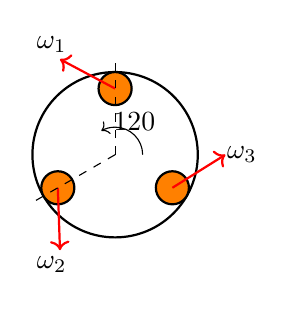
\begin{tikzpicture}[scale=0.7]
    % Ball (top view)
    \draw[thick] (0,0) circle (1.5cm);
    
    % Rollers
    \foreach \angle in {90, 210, 330} {
        \draw[fill=orange, thick] (\angle:1.2cm) circle (0.3cm);
        \draw[->, thick, red] (\angle:1.2cm) -- (\angle+30:2cm);
        \node at (\angle+30:2.3cm) {$\omega_{\pgfmathparse{int((\angle-90)/120+1)}\pgfmathresult}$};
    }
    
    % Angles
    \draw[dashed] (0,0) -- (90:1.8cm);
    \draw[dashed] (0,0) -- (210:1.8cm);
    \draw[->] (0.5,0) arc (0:120:0.5cm);
    \node at (60:0.7cm) {$120°$};
\end{tikzpicture}

\column{0.5\textwidth}
\textbf{Side View}
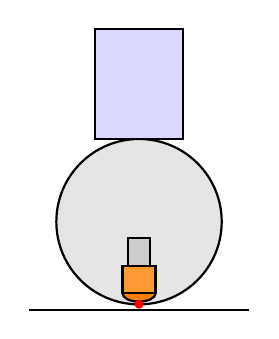
\begin{tikzpicture}[scale=0.7]
    % Ball
    \draw[fill=gray!20, thick] (0,0) circle (1.5cm);
    
    % Body frame
    \draw[fill=blue!15, thick] (-0.8,1.5) rectangle (0.8,3.5);
    
    % Roller
    \draw[fill=orange, thick] (0,-1.3) ellipse (0.3cm and 0.15cm);
    \draw[fill=orange!80, thick] (-0.3,-1.3) -- (-0.3,-0.8) -- (0.3,-0.8) -- (0.3,-1.3) -- cycle;
    
    % Motor
    \draw[fill=gray!40, thick] (-0.2,-0.8) rectangle (0.2,-0.3);
    
    % Contact point
    \fill[red] (0,-1.5) circle (0.08cm);
    
    % Ground
    \draw[thick] (-2,-1.6) -- (2,-1.6);
\end{tikzpicture}
\end{columns}
\note{Three rollers at 120-degree spacing provide omnidirectional control. Each roller is driven by a NEMA17 stepper motor. The symmetric configuration ensures balanced force distribution.}
\end{frame}

\begin{frame}{Center of Mass and IMU Placement}
\begin{columns}
\column{0.6\textwidth}
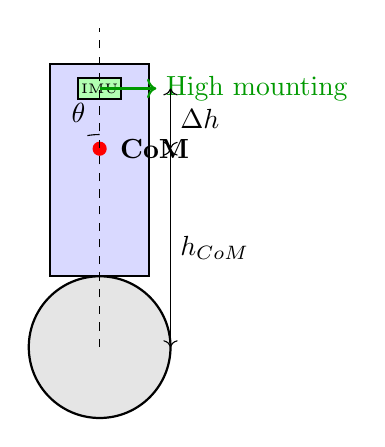
\begin{tikzpicture}[scale=0.9]
    % Ball
    \draw[fill=gray!20, thick] (0,0) circle (1cm);
    
    % Body
    \draw[fill=blue!15, thick] (-0.7,1) rectangle (0.7,4);
    
    % CoM
    \fill[red] (0,2.8) circle (0.1cm);
    \node[right] at (0.15,2.8) {\textbf{CoM}};
    
    % IMU
    \draw[fill=green!30, thick] (-0.3,3.5) rectangle (0.3,3.8);
    \node at (0,3.65) {\tiny IMU};
    \draw[->, thick, green!60!black] (0,3.65) -- (0.8,3.65);
    \node[right, green!60!black] at (0.8,3.65) {High mounting};
    
    % Dimensions
    \draw[<->] (1.0,0) -- (1.0,2.8);
    \node[right] at (1.0,1.4) {$h_{CoM}$};
    
    \draw[<->] (1.0,2.8) -- (1.0,3.65);
    \node[right] at (1.0,3.225) {$\Delta h$};
    
    % Tilt angle
    \draw[dashed] (0,0) -- (0,4.5);
    \draw (0,3) arc (90:100:1);
    \node at (-0.3,3.3) {$\theta$};
\end{tikzpicture}

\column{0.4\textwidth}
\textbf{Design Criteria:}
\begin{itemize}
    \item CoM high above ball center
    \item Increased $h$ $\rightarrow$ longer time constant
    \item IMU near top for better sensitivity
    \item Symmetric mass distribution
\end{itemize}

\vspace{0.5cm}
$$T_{fall} \propto \sqrt{\frac{h}{g}}$$
\end{columns}
\note{Higher center of mass gives more time to react before falling, but also means higher inertia. The IMU is mounted high to maximize angular rate sensitivity during tilt.}
\end{frame}

% Section 3: Hardware Architecture
\section{Hardware Architecture}

\begin{frame}{Electronics Block Diagram}
\begin{center}
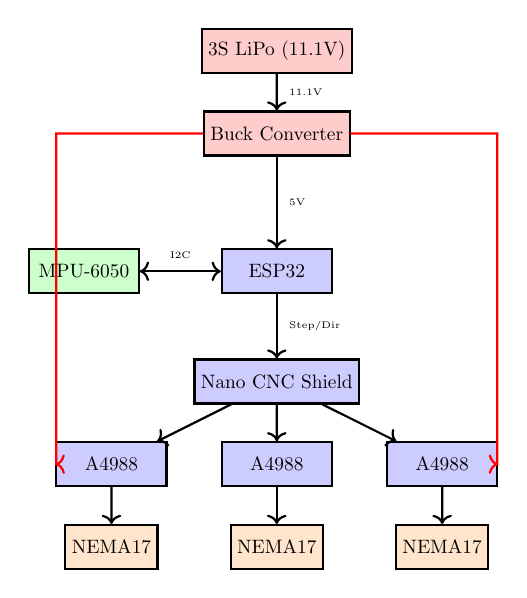
\begin{tikzpicture}[
    block/.style={rectangle, draw, fill=blue!20, thick, minimum height=0.8cm, minimum width=2cm},
    sensor/.style={rectangle, draw, fill=green!20, thick, minimum height=0.8cm, minimum width=2cm},
    power/.style={rectangle, draw, fill=red!20, thick, minimum height=0.8cm, minimum width=2cm},
    motor/.style={rectangle, draw, fill=orange!20, thick, minimum height=0.8cm, minimum width=1.5cm},
    scale=0.7, transform shape
    ]
    
    % Power supply
    \node[power] (battery) at (0,4) {3S LiPo (11.1V)};
    \node[power] (buck) at (0,2.5) {Buck Converter};
    \draw[->, thick] (battery) -- (buck);
    \node[right] at (0.1,3.25) {\tiny 11.1V};
    
    % Controller  
    \node[block] (esp32) at (0,0) {ESP32};
    \draw[->, thick] (buck) -- (esp32);
    \node[right] at (0.1,1.25) {\tiny 5V};
    
    % Sensor
    \node[sensor] (imu) at (-3.5,0) {MPU-6050};
    \draw[<->, thick] (imu) -- (esp32);
    \node[above] at (-1.75,0.1) {\tiny I2C};
    
    % CNC Shield
    \node[block] (shield) at (0,-2) {Nano CNC Shield};
    \draw[->, thick] (esp32) -- (shield);
    \node[right] at (0.1,-1) {\tiny Step/Dir};
    
    % Drivers
    \node[block] (drv1) at (-3,-3.5) {A4988};
    \node[block] (drv2) at (0,-3.5) {A4988};
    \node[block] (drv3) at (3,-3.5) {A4988};
    
    \draw[->, thick] (shield) -- (drv1);
    \draw[->, thick] (shield) -- (drv2);
    \draw[->, thick] (shield) -- (drv3);
    
    % Motors
    \node[motor] (m1) at (-3,-5) {NEMA17};
    \node[motor] (m2) at (0,-5) {NEMA17};
    \node[motor] (m3) at (3,-5) {NEMA17};
    
    \draw[->, thick] (drv1) -- (m1);
    \draw[->, thick] (drv2) -- (m2);
    \draw[->, thick] (drv3) -- (m3);
    
    % Power to drivers
    \draw[->, thick, red] (buck) -| (-4,2.5) -- (-4,-3.5) -- (drv1);
    \draw[->, thick, red] (buck) -| (4,2.5) -- (4,-3.5) -- (drv3);
\end{tikzpicture}
\end{center}
\note{The ESP32 provides the computational power for sensor fusion and control. The CNC shield simplifies the step/direction interface to three A4988 drivers, each controlling a NEMA17 stepper motor.}
\end{frame}

\begin{frame}{Component Specifications}
\begin{table}
\small
\begin{tabular}{lll}
\hline
\textbf{Component} & \textbf{Specification} & \textbf{Purpose} \\
\hline
ESP32 & 240 MHz dual-core & Control + sensor fusion \\
MPU-6050 & 6-axis IMU, 1 kHz max & Tilt measurement \\
A4988 & 2A max, 1/16 microstep & Stepper driver \\
NEMA17 & 1.5A, 0.4 Nm & Roller actuation \\
3S LiPo & 11.1V, 2200 mAh & Power supply \\
Buck Conv. & 11.1V $\rightarrow$ 5V, 3A & Voltage regulation \\
\hline
\end{tabular}
\end{table}

\vspace{0.5cm}
\begin{block}{Key Design Choices}
\begin{itemize}
    \item ESP32: Sufficient speed for real-time control (<10 ms loop)
    \item MPU-6050: Cost-effective 6-DOF with reasonable noise
    \item A4988: Simple step/dir interface, adequate current
\end{itemize}
\end{block}
\note{Component selection balanced performance, cost, and ease of integration. The ESP32's dual-core capability allows separation of sensor reading and control tasks.}
\end{frame}

% Section 4: System Modeling
\section{System Modeling}

\begin{frame}{Coordinate Frames}
\begin{columns}
\column{0.5\textwidth}
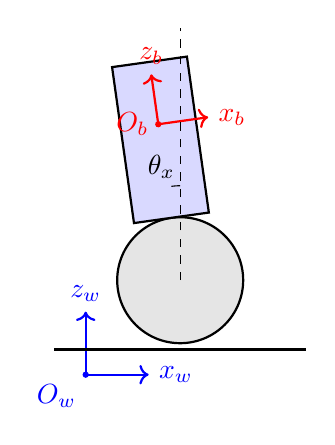
\begin{tikzpicture}[scale=0.8]
    % World frame
    \draw[->, thick, blue] (-1.5,-1.5) -- (-0.5,-1.5) node[right] {$x_w$};
    \draw[->, thick, blue] (-1.5,-1.5) -- (-1.5,-0.5) node[above] {$z_w$};
    \fill[blue] (-1.5,-1.5) circle (0.05cm);
    \node[below left, blue] at (-1.5,-1.5) {$O_w$};
    
    % Ball
    \draw[fill=gray!20, thick] (0,0) circle (1cm);
    
    % Body (tilted)
    \begin{scope}[rotate around={8:(0,0)}]
        \draw[fill=blue!15, thick] (-0.6,1) rectangle (0.6,3.5);
        
        % Body frame
        \draw[->, thick, red] (0,2.5) -- (0.8,2.5) node[right] {$x_b$};
        \draw[->, thick, red] (0,2.5) -- (0,3.3) node[above] {$z_b$};
        \fill[red] (0,2.5) circle (0.05cm);
        \node[left, red] at (0,2.5) {$O_b$};
    \end{scope}
    
    % Tilt angles
    \draw[dashed] (0,0) -- (0,4);
    \draw (0,1.5) arc (90:98:1);
    \node at (-0.3,1.8) {$\theta_x$};
    
    % Ground
    \draw[thick] (-2,-1.1) -- (2,-1.1);
\end{tikzpicture}

\column{0.5\textwidth}
\textbf{Frames:}
\begin{itemize}
    \item World frame: $\{O_w\}$
    \item Body frame: $\{O_b\}$
    \item Ball frame: $\{O_{ball}\}$
\end{itemize}

\vspace{0.3cm}
\textbf{Tilt Angles:}
\begin{align*}
\theta_x &: \text{roll (about } x_w\text{)} \\
\theta_y &: \text{pitch (about } y_w\text{)}
\end{align*}

\vspace{0.3cm}
\textbf{Small Angle Assumption:}
$$|\theta_x|, |\theta_y| < 15°$$
\end{columns}
\note{We define a world-fixed inertial frame and a body-fixed frame that rotates with the robot. The small angle assumption allows linearization of trigonometric functions.}
\end{frame}

\begin{frame}{State and Input Vectors}
\begin{block}{State Vector}
$$\bm{x} = \begin{bmatrix} \theta_x \\ \theta_y \\ \dot{\theta}_x \\ \dot{\theta}_y \end{bmatrix} \in \mathbb{R}^4$$
\begin{itemize}
    \item $\theta_x, \theta_y$: Tilt angles (rad)
    \item $\dot{\theta}_x, \dot{\theta}_y$: Angular velocities (rad/s)
\end{itemize}
\end{block}

\begin{block}{Input Vector}
$$\bm{u} = \begin{bmatrix} \tau_1 \\ \tau_2 \\ \tau_3 \end{bmatrix} \in \mathbb{R}^3$$
\begin{itemize}
    \item $\tau_i$: Torque from motor $i$ (Nm)
\end{itemize}
\end{block}
\note{The state captures the tilt dynamics - the critical variables for maintaining balance. The inputs are the three motor torques. Notice we have 4 states but only 3 inputs - this is the underactuated nature.}
\end{frame}

\begin{frame}{Free Body Diagram}
\begin{center}
\begin{tikzpicture}[scale=1.0]
    % Ball
    \draw[fill=gray!20, thick] (0,0) circle (1cm);
    
    % Body
    \begin{scope}[rotate around={12:(0,0)}]
        \draw[fill=blue!15, thick] (-0.7,1) rectangle (0.7,3.5);
        
        % Center of mass
        \fill[red] (0,2.5) circle (0.08cm);
        \node[right] at (0.1,2.5) {CoM};
        
        % Forces
        % Gravity
        \draw[->, very thick, red] (0,2.5) -- (0,1.3) node[midway, right] {$mg$};
        
        % Normal force from ball
        \draw[->, very thick, blue] (0,1) -- (0,2.2) node[midway, left] {$N$};
        
        % Friction forces at contact
        \draw[->, thick, green!60!black] (0,1) -- (-0.8,1) node[below] {$f_x$};
        
        % Torques from motors (circular arrows)
        \draw[->, thick, orange] (0.5,0.3) arc (0:270:0.2cm);
        \node[right, orange] at (0.7,0.3) {$\tau_i$};
    \end{scope}
    
    % Ground
    \draw[thick] (-2,-1.1) -- (2,-1.1);
    \draw[pattern=north east lines] (-2,-1.1) rectangle (2,-1.3);
    
    % Dimensions
    \draw[<->, dashed] (1.3,0) -- (1.3,2.5);
    \node[right] at (1.3,1.25) {$h$};
    
    % Angle annotation
    \draw[dashed] (0,0) -- (0,4);
    \draw (0,2) arc (90:102:0.5);
    \node at (-0.25,2.3) {$\theta$};
\end{tikzpicture}
\end{center}
\note{The free body diagram shows the key forces: gravity acting at the CoM, normal force from the ball, friction at the ball-body interface, and motor torques. The restoring moment from gravity is what makes the system unstable.}
\end{frame}

% Section 5: Dynamic Equations
\section{Dynamic Equations}

\begin{frame}{Inverted Pendulum Analogy}
\begin{columns}
\column{0.5\textwidth}
\textbf{Linearized Dynamics:}
\begin{align*}
I\ddot{\theta} &= mgh\sin\theta - \tau_{motor} \\
&\approx mgh\theta - \tau_{motor}
\end{align*}

For small angles:
$$\ddot{\theta} = \frac{mgh}{I}\theta - \frac{\tau_{motor}}{I}$$

\vspace{0.3cm}
Define: $\omega_n^2 = \frac{mgh}{I}$ (natural frequency)

$$\ddot{\theta} = \omega_n^2 \theta - \frac{\tau_{motor}}{I}$$

\column{0.5\textwidth}
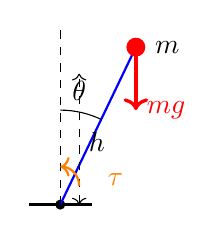
\begin{tikzpicture}[scale=0.8]
    % Pivot
    \fill (0,0) circle (0.08cm);
    \draw[thick] (-0.5,0) -- (0.5,0);
    
    % Pendulum
    \draw[thick, blue] (0,0) -- (1.2,2.5);
    
    % Mass
    \fill[red] (1.2,2.5) circle (0.15cm);
    \node[right] at (1.35,2.5) {$m$};
    
    % Length
    \draw[<->, dashed] (0.3,0) -- (0.3,2.08);
    \node[right] at (0.3,1) {$h$};
    
    % Angle
    \draw[dashed] (0,0) -- (0,2.8);
    \draw (0,1.5) arc (90:64:1.5);
    \node at (0.3,1.8) {$\theta$};
    
    % Gravity
    \draw[->, very thick, red] (1.2,2.5) -- (1.2,1.5) node[right] {$mg$};
    
    % Torque
    \draw[->, thick, orange] (0.3,0.3) arc (0:90:0.3);
    \node[right, orange] at (0.6,0.4) {$\tau$};
\end{tikzpicture}
\end{columns}
\note{The ballbot behaves like an inverted pendulum. Without control torque, the system is unstable with exponentially growing tilt. The motor torque must counteract the destabilizing gravitational moment.}
\end{frame}

\begin{frame}{Torque to Angular Acceleration}
\textbf{Motor torques produce body angular acceleration:}

\begin{equation}
\begin{bmatrix} \ddot{\theta}_x \\ \ddot{\theta}_y \end{bmatrix} = 
\begin{bmatrix} 
\omega_n^2 & 0 \\ 
0 & \omega_n^2 
\end{bmatrix}
\begin{bmatrix} \theta_x \\ \theta_y \end{bmatrix}
+ \frac{1}{I} \bm{J}_{motor} 
\begin{bmatrix} \tau_1 \\ \tau_2 \\ \tau_3 \end{bmatrix}
\end{equation}

where $\bm{J}_{motor}$ maps motor torques to body angular accelerations.

\vspace{0.5cm}
\textbf{For 120° configuration:}
$$\bm{J}_{motor} = \frac{r_{ball}}{3}
\begin{bmatrix}
0 & -\sqrt{3}/2 & \sqrt{3}/2 \\
1 & -1/2 & -1/2
\end{bmatrix}$$

where $r_{ball}$ is the ball radius.
\note{The Jacobian matrix transforms the three motor torques into two-dimensional angular acceleration. The 120-degree spacing creates this specific mapping.}
\end{frame}

\begin{frame}{Tilt to Translation Relationship}
\textbf{Controlled tilt produces ball motion:}

$$\ddot{\bm{p}}_{ball} = g \begin{bmatrix} \tan\theta_y \\ -\tan\theta_x \end{bmatrix} \approx g \begin{bmatrix} \theta_y \\ -\theta_x \end{bmatrix}$$

\vspace{0.3cm}
\textbf{Principle:}
\begin{itemize}
    \item Tilt forward $(\theta_y > 0)$ $\rightarrow$ ball rolls forward
    \item Tilt right $(\theta_x > 0)$ $\rightarrow$ ball rolls right
    \item Acceleration proportional to tilt angle
\end{itemize}

\vspace{0.3cm}
\begin{block}{Control Strategy}
To move in direction $\bm{v}_{desired}$:
\begin{enumerate}
    \item Command tilt: $\theta_{cmd} = k_v \bm{v}_{desired}$
    \item Maintain tilt via motor torques
    \item Ball accelerates in desired direction
\end{enumerate}
\end{block}
\note{This is the key insight for locomotion: by maintaining a controlled tilt, we induce acceleration in the desired direction. The system must continuously balance while achieving this tilt.}
\end{frame}

\begin{frame}{Simplified Nonlinear Model}
\textbf{Complete MIMO underactuated dynamics:}

\begin{align*}
\dot{\bm{x}} &= \bm{f}(\bm{x}, \bm{u}) \\[0.3cm]
\begin{bmatrix} \dot{\theta}_x \\ \dot{\theta}_y \\ \ddot{\theta}_x \\ \ddot{\theta}_y \end{bmatrix}
&= \begin{bmatrix} 
\dot{\theta}_x \\ 
\dot{\theta}_y \\ 
\omega_n^2 \sin\theta_x - \frac{c_1\tau_1 + c_2\tau_2 + c_3\tau_3}{I} \\
\omega_n^2 \sin\theta_y - \frac{d_1\tau_1 + d_2\tau_2 + d_3\tau_3}{I}
\end{bmatrix}
\end{align*}

where $c_i, d_i$ are kinematic coefficients from $\bm{J}_{motor}$.

\vspace{0.3cm}
\textbf{Linearized (small angles):}
$$\dot{\bm{x}} = \bm{A}\bm{x} + \bm{B}\bm{u}$$
\note{The nonlinear model includes sine terms. For control design, we linearize around the upright equilibrium, which is valid for small deviations. This enables linear control techniques like PID.}
\end{frame}

% Section 6: Omni Kinematics
\section{Omni Kinematics}

\begin{frame}{Three-Wheel Kiwi Drive Kinematics}
\begin{columns}
\column{0.5\textwidth}
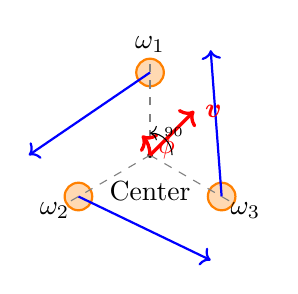
\begin{tikzpicture}[scale=0.7]
    % Ball center
    \fill (0,0) circle (0.05cm);
    \node[below] at (0,-0.3) {Center};
    
    % Wheels at 120°
    \foreach \angle/\label in {90/1, 210/2, 330/3} {
        \draw[thick, orange, fill=orange!30] (\angle:1.5) circle (0.25);
        \node at (\angle:2) {$\omega_{\label}$};
        
        % Velocity vectors
        \draw[->, thick, blue] (\angle:1.5) -- (\angle+90:2.2);
        
        % Angle lines
        \draw[dashed, gray] (0,0) -- (\angle:1.8);
    }
    
    % Global velocity
    \draw[->, very thick, red] (0,0) -- (0.8,0.8) node[right] {$\bm{v}$};
    \draw[->, very thick, red] (0,0) arc (0:45:0.5);
    \node[red] at (0.3,0.15) {$\phi$};
    
    % Angles
    \draw[->] (0.4,0) arc (0:90:0.4);
    \node at (45:0.6) {\tiny $90°$};
\end{tikzpicture}

\column{0.5\textwidth}
\textbf{Velocity decomposition:}

Global velocity:
$$\bm{v} = \begin{bmatrix} v_x \\ v_y \end{bmatrix}$$

Angular velocity: $\omega_r$ (rotation)

\vspace{0.3cm}
\textbf{Goal:}
Find $[\omega_1, \omega_2, \omega_3]^T$ to achieve $\bm{v}$ and $\omega_r$
\end{columns}
\note{Each roller can only push perpendicular to its mounting direction. Three rollers at 120 degrees provide omnidirectional mobility through proper velocity decomposition.}
\end{frame}

\begin{frame}{Inverse Kinematics Derivation}
\textbf{Velocity at wheel $i$ perpendicular to mounting:}
$$v_{\perp,i} = \bm{v} \cdot \bm{n}_i + r_{config} \omega_r$$

where $\bm{n}_i$ is the unit normal vector for wheel $i$.

\vspace{0.3cm}
\textbf{For 120° configuration:}
\begin{align*}
\bm{n}_1 &= \begin{bmatrix} -1 \\ 0 \end{bmatrix}, \quad
\bm{n}_2 = \begin{bmatrix} 1/2 \\ -\sqrt{3}/2 \end{bmatrix}, \quad
\bm{n}_3 = \begin{bmatrix} 1/2 \\ \sqrt{3}/2 \end{bmatrix}
\end{align*}

\textbf{Wheel angular velocity:}
$$\omega_i = \frac{v_{\perp,i}}{r_{roller}}$$
\note{Each roller velocity is the projection of the body velocity onto the roller's perpendicular direction, plus a contribution from body rotation.}
\end{frame}

\begin{frame}{Matrix Form}
\textbf{Inverse kinematics (body to wheels):}
$$\begin{bmatrix} \omega_1 \\ \omega_2 \\ \omega_3 \end{bmatrix} = 
\frac{1}{r_{roller}}
\begin{bmatrix}
-1 & 0 & r_{config} \\
1/2 & -\sqrt{3}/2 & r_{config} \\
1/2 & \sqrt{3}/2 & r_{config}
\end{bmatrix}
\begin{bmatrix} v_x \\ v_y \\ \omega_r \end{bmatrix}$$

\vspace{0.5cm}
Compact form:
$$\bm{\omega}_{wheels} = \bm{J}^{-1} \bm{v}_{body}$$

\vspace{0.5cm}
\textbf{Note:} For ballbot, $\omega_r$ is typically set to 0 (no body spin).

\textbf{Usage:} Desired tilt $\bm{\theta}_{cmd}$ $\rightarrow$ $\bm{v}_{body}$ $\rightarrow$ $\bm{\omega}_{wheels}$
\note{This matrix equation is implemented in software to convert commanded body velocities into individual motor speeds. The controller adjusts these speeds in real-time to maintain balance and achieve motion.}
\end{frame}

% Section 7: Control System Design
\section{Control System Design}

\begin{frame}{Sensor Fusion: Complementary Filter}
\textbf{MPU-6050 provides:}
\begin{itemize}
    \item Accelerometer: Tilt estimate (noisy, no drift)
    \item Gyroscope: Angular rate (clean, but drifts)
\end{itemize}

\vspace{0.3cm}
\textbf{Complementary filter:}
$$\theta_{fused}[k] = \alpha \cdot (\theta_{fused}[k-1] + \omega_{gyro} \cdot dt) + (1-\alpha) \cdot \theta_{accel}$$

where:
\begin{itemize}
    \item $\alpha \approx 0.98$ (high-pass on gyro, low-pass on accel)
    \item $dt$: Sample period
    \item $\theta_{accel} = \text{atan2}(a_y, a_z)$ for roll
\end{itemize}

\vspace{0.3cm}
\begin{block}{Why Complementary Filter?}
\begin{itemize}
    \item Simple, computationally efficient
    \item Real-time suitable (Kalman filter is better but more complex)
    \item Sufficient for ballbot application
\end{itemize}
\end{block}
\note{The complementary filter trusts the gyroscope for short-term changes and the accelerometer for long-term absolute reference. This provides a drift-free, low-noise tilt estimate critical for control.}
\end{frame}

\begin{frame}{PID Control Structure}
\textbf{Independent PID for each axis:}

$$\tau_i = K_p e + K_i \int e \, dt + K_d \frac{de}{dt}$$

where $e = \theta_{setpoint} - \theta_{measured}$

\vspace{0.3cm}
\textbf{Discrete implementation:}
\begin{align*}
P[k] &= K_p \cdot e[k] \\
I[k] &= I[k-1] + K_i \cdot e[k] \cdot dt \\
D[k] &= K_d \cdot \frac{e[k] - e[k-1]}{dt} \\
u[k] &= P[k] + I[k] + D[k]
\end{align*}

\textbf{Anti-windup:} Clamp $I[k]$ to prevent integral saturation
\note{Each axis (roll and pitch) has its own PID controller. The proportional term provides immediate response, derivative term damping, and integral term eliminates steady-state error.}
\end{frame}

\begin{frame}{Control Block Diagram}
\begin{center}
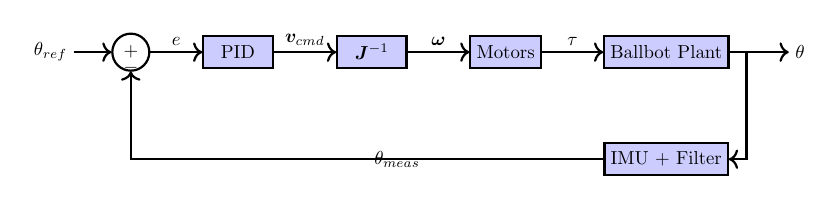
\begin{tikzpicture}[
    block/.style={rectangle, draw, fill=blue!20, thick, minimum height=0.6cm, minimum width=1.3cm},
    sum/.style={circle, draw, thick, minimum size=0.5cm},
    scale=0.68, every node/.style={scale=0.68}
    ]
    
    % Input
    \node (input) at (-6,0) {$\theta_{ref}$};
    
    % Summing junction
    \node[sum] (sum1) at (-4.5,0) {$+$};
    \node at (-4.5,-0.3) {$-$};
    \draw[->, thick] (input) -- (sum1);
    
    % PID controller
    \node[block] (pid) at (-2.5,0) {PID};
    \draw[->, thick] (sum1) -- (pid) node[midway, above] {$e$};
    
    % Kinematic mapping
    \node[block] (kin) at (0,0) {$\bm{J}^{-1}$};
    \draw[->, thick] (pid) -- (kin) node[midway, above] {$\bm{v}_{cmd}$};
    
    % Motors
    \node[block] (motors) at (2.5,0) {Motors};
    \draw[->, thick] (kin) -- (motors) node[midway, above] {$\bm{\omega}$};
    
    % Plant (physical system)
    \node[block, minimum width=1.8cm] (plant) at (5.5,0) {Ballbot Plant};
    \draw[->, thick] (motors) -- (plant) node[midway, above] {$\tau$};
    
    % Output
    \node (output) at (8,0) {$\theta$};
    \draw[->, thick] (plant) -- (output);
    
    % Sensor
    \node[block] (sensor) at (5.5,-2) {IMU + Filter};
    \draw[->, thick] (7,0) |- (sensor);
    
    % Feedback
    \draw[->, thick] (sensor) -| (sum1) node[pos=0.25, right] {$\theta_{meas}$};
    
\end{tikzpicture}
\end{center}
\note{This closed-loop control system continuously measures tilt, compares to reference, computes control action via PID, converts to motor commands via inverse kinematics, and actuates the motors.}
\end{frame}

\begin{frame}{Tilt-Based Locomotion Control}
\textbf{Locomotion via tilt reference:}

To move with velocity $\bm{v}_{desired}$:
$$\theta_{ref} = K_{locomotion} \cdot \bm{v}_{desired}$$

\vspace{0.3cm}
\begin{columns}
\column{0.5\textwidth}
\textbf{Example:}
\begin{itemize}
    \item Move forward: $\theta_{y,ref} = +0.1$ rad
    \item Move right: $\theta_{x,ref} = +0.1$ rad
    \item Stop: $\theta_{ref} = 0$
\end{itemize}

\column{0.5\textwidth}
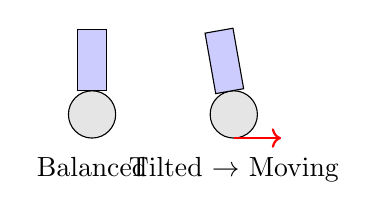
\begin{tikzpicture}[scale=0.6]
    % Before
    \draw[fill=gray!20] (0,0) circle (0.5);
    \draw[fill=blue!20] (-0.3,0.5) rectangle (0.3,1.8);
    \node[below] at (0,-0.7) {Balanced};
    
    % After
    \begin{scope}[xshift=3cm]
        \draw[fill=gray!20] (0,0) circle (0.5);
        \begin{scope}[rotate=10]
            \draw[fill=blue!20] (-0.3,0.5) rectangle (0.3,1.8);
        \end{scope}
        \draw[->, thick, red] (0,-0.5) -- (1,-0.5);
        \node[below] at (0,-0.7) {Tilted $\rightarrow$ Moving};
    \end{scope}
\end{tikzpicture}
\end{columns}

\vspace{0.3cm}
\textbf{Control loop:}
Outer loop (locomotion) sets $\theta_{ref}$ $\rightarrow$ Inner loop (balance) maintains tilt
\note{Locomotion is achieved through a cascaded control structure. The outer loop determines desired tilt for motion, while the inner loop (PID) maintains that tilt against disturbances.}
\end{frame}

% Section 8: Software Architecture
\section{Software Architecture}

\begin{frame}{Control Loop Structure}
\begin{columns}
\column{0.5\textwidth}
\textbf{Main Control Loop:}
\begin{enumerate}
    \item Read IMU (I2C)
    \item Complementary filter
    \item Compute PID
    \item Inverse kinematics
    \item Send step pulses
    \item \textcolor{blue}{Repeat at fixed rate}
\end{enumerate}

\vspace{0.3cm}
\textbf{Timing Requirements:}
\begin{itemize}
    \item Loop frequency: 100-200 Hz
    \item Jitter: $<$ 1 ms
    \item Total latency: $<$ 10 ms
\end{itemize}

\column{0.5\textwidth}
\textbf{ESP32 Task Separation:}

Core 0:
\begin{itemize}
    \item Sensor reading
    \item Filter update
\end{itemize}

Core 1:
\begin{itemize}
    \item Control computation
    \item Motor commands
    \item Communication
\end{itemize}

\vspace{0.3cm}
Uses FreeRTOS for task management
\end{columns}
\note{Dual-core architecture allows parallel processing: one core handles time-critical sensor acquisition, the other handles control computation. This ensures consistent loop timing.}
\end{frame}

\begin{frame}{Software Flow Diagram}
\begin{center}
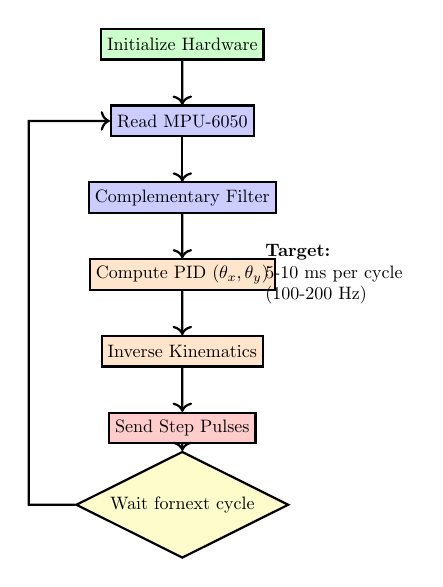
\begin{tikzpicture}[
    block/.style={rectangle, draw, thick, minimum width=2.8cm, minimum height=0.6cm},
    decision/.style={diamond, draw, thick, aspect=2, minimum width=1.8cm},
    scale=0.65, every node/.style={scale=0.65}
    ]
    
    % Start
    \node[block, fill=green!20] (start) at (0,0) {Initialize Hardware};
    
    % Read sensor
    \node[block, fill=blue!20] (read) at (0,-1.5) {Read MPU-6050};
    \draw[->, thick] (start) -- (read);
    
    % Filter
    \node[block, fill=blue!20] (filter) at (0,-3) {Complementary Filter};
    \draw[->, thick] (read) -- (filter);
    
    % PID
    \node[block, fill=orange!20] (pid) at (0,-4.5) {Compute PID ($\theta_x, \theta_y$)};
    \draw[->, thick] (filter) -- (pid);
    
    % Kinematics
    \node[block, fill=orange!20] (kin) at (0,-6) {Inverse Kinematics};
    \draw[->, thick] (pid) -- (kin);
    
    % Motor command
    \node[block, fill=red!20] (motor) at (0,-7.5) {Send Step Pulses};
    \draw[->, thick] (kin) -- (motor);
    
    % Delay
    \node[decision, fill=yellow!20] (delay) at (0,-9) {Wait for\\next cycle};
    \draw[->, thick] (motor) -- (delay);
    
    % Loop back
    \draw[->, thick] (delay) -- (-3,-9) -- (-3,-1.5) -- (read);
    
    % Timing annotation
    \node[right, text width=2.8cm] at (1.5,-4.5) {\textbf{Target:}\\5-10 ms per cycle\\(100-200 Hz)};
    
\end{tikzpicture}
\end{center}
\note{This flowchart shows the sequential execution of the control loop. Each iteration must complete within the target cycle time to maintain stability.}
\end{frame}

% Section 9: Power and Drivers
\section{Power and Driver Calculations}

\begin{frame}{A4988 Current Limiting}
\textbf{Setting motor current via reference voltage:}

$$I_{max} = \frac{V_{ref}}{8 \cdot R_{sense}}$$

For A4988 with $R_{sense} = 0.1\, \Omega$:
$$I_{max} = \frac{V_{ref}}{0.8}$$

\vspace{0.3cm}
\textbf{Example calculation:}
\begin{itemize}
    \item NEMA17 rated current: $I_{rated} = 1.5$ A
    \item Set to 70\% for margin: $I_{set} = 1.05$ A
    \item Required $V_{ref}$: $V_{ref} = 0.8 \times 1.05 = 0.84$ V
\end{itemize}

\vspace{0.3cm}
\textbf{Adjustment:} Use small screwdriver on potentiometer while measuring $V_{ref}$ with multimeter
\note{Proper current limiting is critical to prevent motor overheating and driver damage. Too low and you lose torque; too high and components overheat.}
\end{frame}

\begin{frame}{Power Consumption and Battery Life}
\textbf{Power budget:}
\begin{align*}
P_{motors} &= 3 \times V_{supply} \times I_{avg} = 3 \times 11.1 \times 0.8 = 26.6\text{ W} \\
P_{electronics} &\approx 2\text{ W} \\
P_{total} &\approx 29\text{ W}
\end{align*}

\vspace{0.3cm}
\textbf{Battery discharge:}

For 3S LiPo, 2200 mAh at 11.1V:
$$E_{battery} = 2.2 \times 11.1 = 24.4\text{ Wh}$$

Estimated runtime:
$$t_{run} = \frac{24.4}{29} \times 0.8 \approx 40\text{ minutes}$$

(Factor 0.8 accounts for inefficiency and voltage drop)
\note{Battery life depends on usage pattern. Aggressive maneuvering draws more current. Always monitor battery voltage to prevent over-discharge which can damage LiPo cells.}
\end{frame}

% Section 10: Stability and Tuning
\section{Stability and Tuning}

\begin{frame}{PID Gain Selection Effects}
\begin{table}
\small
\begin{tabular}{llll}
\hline
\textbf{Gain} & \textbf{Too Low} & \textbf{Too High} & \textbf{Effect} \\
\hline
$K_p$ & Slow response & Oscillation & Proportional \\
$K_i$ & Steady error & Windup, overshoot & Eliminates bias \\
$K_d$ & Overshoot & Noise amplification & Damping \\
\hline
\end{tabular}
\end{table}

\vspace{0.5cm}
\textbf{Tuning procedure:}
\begin{enumerate}
    \item Start with all gains at zero
    \item Increase $K_p$ until small oscillations appear
    \item Add $K_d$ to dampen oscillations
    \item Add small $K_i$ to eliminate steady-state error
    \item Fine-tune iteratively
\end{enumerate}

\vspace{0.3cm}
\textbf{Typical values (normalized):}
$$K_p \approx 10\text{-}50, \quad K_i \approx 0.1\text{-}1, \quad K_d \approx 1\text{-}5$$
\note{PID tuning is iterative and system-specific. Start conservative and increase gains gradually. Test in safe environment with fall protection.}
\end{frame}

\begin{frame}{Oscillation Analysis}
\begin{columns}
\column{0.5\textwidth}
\textbf{Types of oscillation:}

\textbf{1. High-frequency ($>$ 10 Hz):}
\begin{itemize}
    \item Cause: Excessive $K_d$
    \item Fix: Reduce $K_d$, add filter
\end{itemize}

\textbf{2. Medium frequency (2-5 Hz):}
\begin{itemize}
    \item Cause: Excessive $K_p$
    \item Fix: Reduce $K_p$, increase $K_d$
\end{itemize}

\textbf{3. Low frequency ($<$ 1 Hz):}
\begin{itemize}
    \item Cause: Excessive $K_i$
    \item Fix: Reduce $K_i$, add anti-windup
\end{itemize}

\column{0.5\textwidth}
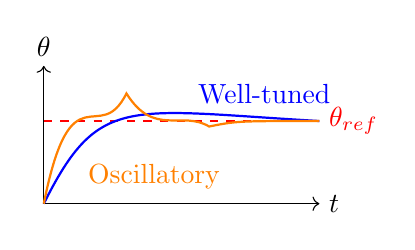
\begin{tikzpicture}[scale=0.7]
    % Stable response
    \draw[->] (0,0) -- (5,0) node[right] {$t$};
    \draw[->] (0,0) -- (0,2.5) node[above] {$\theta$};
    
    % Reference line
    \draw[dashed, red] (0,1.5) -- (5,1.5) node[right] {$\theta_{ref}$};
    
    % Responses
    % Well-tuned
    \draw[thick, blue] (0,0) .. controls (1,2) and (1.5,1.7) .. (5,1.5);
    \node[blue] at (4,2) {Well-tuned};
    
    % Oscillatory
    \draw[thick, orange] (0,0) .. controls (0.5,2.5) and (1,1) .. 
                                  (1.5,2) .. controls (2,1.2) and (2.5,1.7) ..
                                  (3,1.4) .. controls (3.5,1.5) .. (5,1.5);
    \node[orange] at (2,0.5) {Oscillatory};
\end{tikzpicture}
\end{columns}
\note{Oscillations indicate instability or poor tuning. Analyze the frequency and amplitude to diagnose which gain needs adjustment. Always change one parameter at a time.}
\end{frame}

\begin{frame}{Step Response Characteristics}
\begin{center}
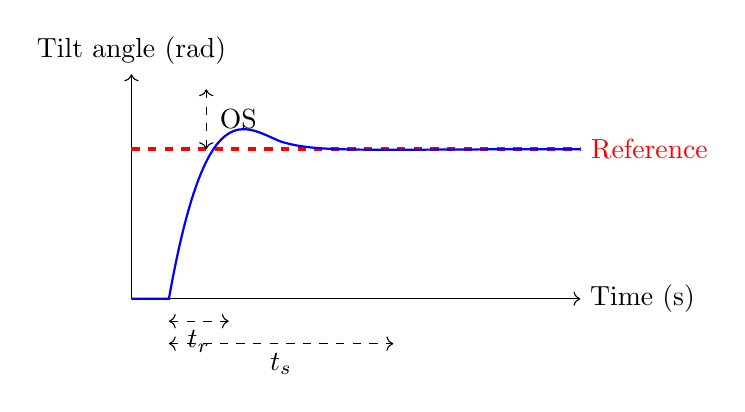
\begin{tikzpicture}[scale=0.95]
    \draw[->] (0,0) -- (6,0) node[right] {Time (s)};
    \draw[->] (0,0) -- (0,3) node[above] {Tilt angle (rad)};
    
    % Reference
    \draw[dashed, red, very thick] (0,2) -- (6,2) node[right] {Reference};
    
    % Response curve
    \draw[thick, blue] (0,0) -- (0.5,0) .. controls (1,2.8) and (1.5,2.3) .. 
                        (2,2.1) .. controls (2.5,1.95) and (3,2) .. (6,2);
    
    % Annotations
    % Rise time
    \draw[<->, dashed] (0.5,-0.3) -- (1.3,-0.3);
    \node[below] at (0.9,-0.3) {$t_r$};
    
    % Overshoot
    \draw[<->, dashed] (1,2) -- (1,2.8);
    \node[right] at (1.05,2.4) {OS};
    
    % Settling time
    \draw[<->, dashed] (0.5,-0.6) -- (3.5,-0.6);
    \node[below] at (2,-0.6) {$t_s$};
    
    % Steady-state error
    \draw[dashed, gray] (5.5,2) -- (5.5,2);
    
\end{tikzpicture}
\end{center}

\textbf{Performance metrics:}
\begin{itemize}
    \item Rise time ($t_r$): Time to reach 90\% of reference
    \item Overshoot (OS): Peak value beyond reference
    \item Settling time ($t_s$): Time to stay within $\pm$2\% of reference
    \item Steady-state error: Final error at $t \rightarrow \infty$
\end{itemize}
\note{Step response analysis helps quantify controller performance. Aim for fast rise time with minimal overshoot and zero steady-state error.}
\end{frame}

% Section 11: Limitations and Extensions
\section{Limitations and Extensions}

\begin{frame}{Current System Limitations}
\begin{block}{Modeling Simplifications}
\begin{itemize}
    \item Small angle approximation breaks down at $>$15°
    \item Neglected friction (ball-roller, bearing, aerodynamic)
    \item Assumed rigid body (ignores flexibility)
    \item No slip modeling (critical for rapid maneuvers)
\end{itemize}
\end{block}

\begin{block}{Hardware Constraints}
\begin{itemize}
    \item Stepper motor limitations (torque ripple, finite step size)
    \item IMU noise and bias drift
    \item Computational latency in ESP32
    \item Power constraints (battery weight vs. capacity)
\end{itemize}
\end{block}

\begin{block}{Control Limitations}
\begin{itemize}
    \item PID cannot optimize for multiple objectives
    \item No explicit state estimation (Kalman filter better)
    \item Fixed gains (no adaptive control)
\end{itemize}
\end{block}
\note{Understanding limitations is crucial for realistic expectations and identifying improvement opportunities. Many of these can be addressed with more advanced techniques.}
\end{frame}

\begin{frame}{Friction and Slip Modeling}
\textbf{Friction torque at ball-roller interface:}
$$\tau_{friction} = \mu N r_{contact}$$

where:
\begin{itemize}
    \item $\mu$: Coefficient of friction (rubber on ball)
    \item $N$: Normal force at contact
    \item $r_{contact}$: Contact radius
\end{itemize}

\vspace{0.3cm}
\textbf{Slip condition:}

Slip occurs when commanded torque exceeds maximum static friction:
$$|\tau_{cmd}| > \tau_{friction,max}$$

\textbf{Effects of slip:}
\begin{itemize}
    \item Loss of position tracking
    \item Reduced control authority
    \item Potential instability
\end{itemize}

\textbf{Mitigation:}
\begin{itemize}
    \item High-friction roller materials
    \item Limit maximum acceleration
    \item Slip detection and compensation
\end{itemize}
\note{Slip is a major practical issue during aggressive maneuvers. It violates the no-slip assumption in our kinematic model, causing position drift and control degradation.}
\end{frame}

\begin{frame}{Advanced Control: LQR}
\textbf{Linear Quadratic Regulator (LQR):}

Minimize cost function:
$$J = \int_0^\infty (\bm{x}^T \bm{Q} \bm{x} + \bm{u}^T \bm{R} \bm{u}) \, dt$$

where:
\begin{itemize}
    \item $\bm{Q}$: State cost matrix (penalize deviations)
    \item $\bm{R}$: Input cost matrix (penalize control effort)
\end{itemize}

\vspace{0.3cm}
\textbf{Optimal control law:}
$$\bm{u}^* = -\bm{K} \bm{x}$$

where $\bm{K}$ is computed by solving the Riccati equation.

\vspace{0.3cm}
\textbf{Advantages over PID:}
\begin{itemize}
    \item Systematic design (no manual tuning)
    \item Multi-objective optimization
    \item Provable stability guarantees
\end{itemize}
\note{LQR provides optimal linear control for our linearized system. It automatically balances state regulation and control effort based on designer-specified weights.}
\end{frame}

\begin{frame}{State Estimation: Kalman Filter}
\textbf{Extended Kalman Filter (EKF):}

Handles sensor noise and bias:
$$\hat{\bm{x}}[k|k] = \hat{\bm{x}}[k|k-1] + \bm{K}[k](\bm{z}[k] - \bm{h}(\hat{\bm{x}}[k|k-1]))$$

where:
\begin{itemize}
    \item $\hat{\bm{x}}$: State estimate
    \item $\bm{z}$: Sensor measurements
    \item $\bm{K}$: Kalman gain
    \item $\bm{h}(\cdot)$: Measurement model
\end{itemize}

\vspace{0.3cm}
\textbf{Benefits:}
\begin{itemize}
    \item Optimal fusion of accel and gyro
    \item Bias estimation and correction
    \item Better than complementary filter
    \item Can estimate ball position/velocity
\end{itemize}

\textbf{Trade-off:} Computational complexity
\note{The Kalman filter provides statistically optimal state estimation by properly accounting for sensor noise characteristics. This can significantly improve control performance, especially for position tracking.}
\end{frame}

\begin{frame}{Field-Oriented Control (FOC) for Motors}
\textbf{Upgrading from steppers to BLDC with FOC:}

\begin{columns}
\column{0.5\textwidth}
\textbf{Advantages:}
\begin{itemize}
    \item Smooth torque output
    \item Higher efficiency
    \item Better dynamic response
    \item Torque control mode
    \item Higher speed capability
\end{itemize}

\column{0.5\textwidth}
\textbf{Requirements:}
\begin{itemize}
    \item Current sensing
    \item Rotor position encoder
    \item FOC algorithm
    \item Dedicated motor driver
    \item Higher computational load
\end{itemize}
\end{columns}

\vspace{0.3cm}
\textbf{FOC enables:}
\begin{itemize}
    \item Direct torque control (better than velocity control)
    \item Force/impedance control
    \item Smoother motion
\end{itemize}
\note{Field-oriented control transforms the three-phase motor into a simpler equivalent model where torque and flux can be controlled independently, providing much better dynamic performance.}
\end{frame}

\begin{frame}{Future Work and Extensions}
\begin{columns}
\column{0.5\textwidth}
\textbf{Immediate improvements:}
\begin{itemize}
    \item Implement EKF
    \item Add slip detection
    \item Vibration damping
    \item Remote control interface
    \item Data logging
\end{itemize}

\textbf{Medium-term:}
\begin{itemize}
    \item Switch to LQR/LQG
    \item Add vision system
    \item Autonomous navigation
    \item Path planning
\end{itemize}

\column{0.5\textwidth}
\textbf{Advanced features:}
\begin{itemize}
    \item Machine learning for disturbance rejection
    \item Adaptive control
    \item Multi-robot coordination
    \item Human-robot interaction
\end{itemize}

\textbf{Hardware upgrades:}
\begin{itemize}
    \item BLDC with FOC
    \item Better IMU (BMI088)
    \item Onboard computer (Jetson Nano)
    \item LiDAR for obstacle avoidance
\end{itemize}
\end{columns}
\note{The ballbot platform provides rich opportunities for research and development across control theory, robotics, and AI. Each extension builds on the fundamental balance control we've established.}
\end{frame}

% Conclusion
\section{Conclusion}

\begin{frame}{Summary}
\textbf{Key Takeaways:}
\begin{enumerate}
    \item Ballbot is an underactuated, inherently unstable system
    \item Requires careful mechanical design (120° roller config, high CoM)
    \item Mathematical modeling enables systematic control design
    \item Sensor fusion (complementary filter) provides reliable state estimate
    \item PID control provides balance; tilt commands enable locomotion
    \item Hardware selection balances performance, cost, complexity
    \item Many opportunities for advanced control and AI integration
\end{enumerate}

\vspace{0.5cm}
\begin{block}{Core Principle}
\centering
\textit{Maintain controlled instability to achieve dynamic stability}
\end{block}
\note{The ballbot embodies key concepts in robotics: dynamics, control, sensor fusion, and actuation. Success requires integration across all these domains.}
\end{frame}

\begin{frame}{References and Resources}
\textbf{Key Papers:}
\begin{itemize}
    \item Lauwers et al., "A Dynamically Stable Single-Wheeled Mobile Robot with Inverse Mouse-Ball Drive" (2006)
    \item Kumagai and Ochiai, "Development of a Robot Balancing on a Ball" (2010)
\end{itemize}

\vspace{0.3cm}
\textbf{Software/Hardware:}
\begin{itemize}
    \item ESP32 Arduino Core: \texttt{github.com/espressif/arduino-esp32}
    \item MPU6050 Library: \texttt{github.com/jrowberg/i2cdevlib}
    \item Stepper control: AccelStepper library
\end{itemize}

\vspace{0.3cm}
\textbf{Further Learning:}
\begin{itemize}
    \item Slotine \& Li, "Applied Nonlinear Control"
    \item Åström \& Murray, "Feedback Systems"
    \item Lynch \& Park, "Modern Robotics"
\end{itemize}
\note{These resources provide deeper mathematical treatment and practical implementation guidance for those interested in building their own ballbot system.}
\end{frame}

\begin{frame}
\begin{center}
{\Huge Thank You!}

\vspace{1cm}
{\Large Questions?}

\vspace{2cm}
\texttt{Contact: cipher0xx@gmail.com}
\end{center}
\note{Thank you for your attention. I'm happy to answer questions about any aspect of the design, implementation, or theory behind this ballbot system.}
\end{frame}

\end{document}